\subsection{Länge des kürzesten Pfades}

Die Breitensuche ist nicht nur ein Verfahren, um Knoten in einem Graphen systematisch aufzulisten. Dank der speziellen Reihernfolge, in der die Knoten besucht werden (zuerst die direkten Nachbarn, dann dessen Nachbarn und so weiter), sind wir sicher, dass wir jeden erreichbaren Knoten über einen kürzesten Pfad erreichen. In diesem Abschnitt werden wir den Algorithmus, den wir im vorherigen Abschnitt kennengelernt haben, so erweitern, dass wir auch den Abstand zwischen zwei Knoten in einem Graphen berechnen können.

Wie wir schon wissen, der Abstand zwischen zwei Knoten ist definiert als die Länge des kürzesten Pfades zwischen diesen zwei Knoten. Ein Pfad ist eine Folge von Knoten, die, wie eine Kette, eine Kante zum vorherigen und zum nächsten Knoten haben. Formal hatten wir den Pfad wie folgt definiert.

\begin{definition}
Sei \(G = (V,E)\) ein ungerichteter Graph. Ein \textbf{Pfad} \(P = {v_0, v_1, \dots, v_n}\) der Länge \(n\) ist eine Folge von paarweise verschiedenen Knoten \(v_i \in V\) so dass zwischen zwei darauffolgenden Knoten eine Kante verläuft, d.h. \({v_i, v_{i+1}} \in E\) für alle i \(\in {0, n-1}\).
\end{definition}

Der kürzeste Pfad zwichen zwei Knoten \(u\) und \(v\) ist der Pfad mit der kleinsten Länge dessen Endknoten \(u\) und \(v\) sind.

\begin{aufgabe}
Zeichne einen vollständigen Graphen mit 5 Knoten. Was ist die Länge des kürzesten Pfades zwischen zwei beliebigen Knoten?
\end{aufgabe}
\begin{aufgabe}
Zeichne einen Gittergraphen mit 2 mal 3 Knoten. Welche zwei Knoten sind am weitesten auseinander? Bestimme den Abstand (die Länge des kürzesten Pfades) zwischen diesen zwei Knoten.
\end{aufgabe}
\begin{aufgabe}
Zeichne einen Kreis mit 6 Knoten. Welche zwei Knoten sind am weitesten auseinander? Wie weit sind sie voneinander entfernt?
\end{aufgabe}

\paragraph{Das Wikipedia-Spiel}
Der Wikipedia-Graph ist nicht so übersichtlich und regelmässig, wie die Graphen, die wir gerade gesehen haben. Um den kürzesten Pfad zwischen zwei Artikel zu finden, muss Bob systematisch vorgehen. 
\begin{figure}[h]
    \centering
    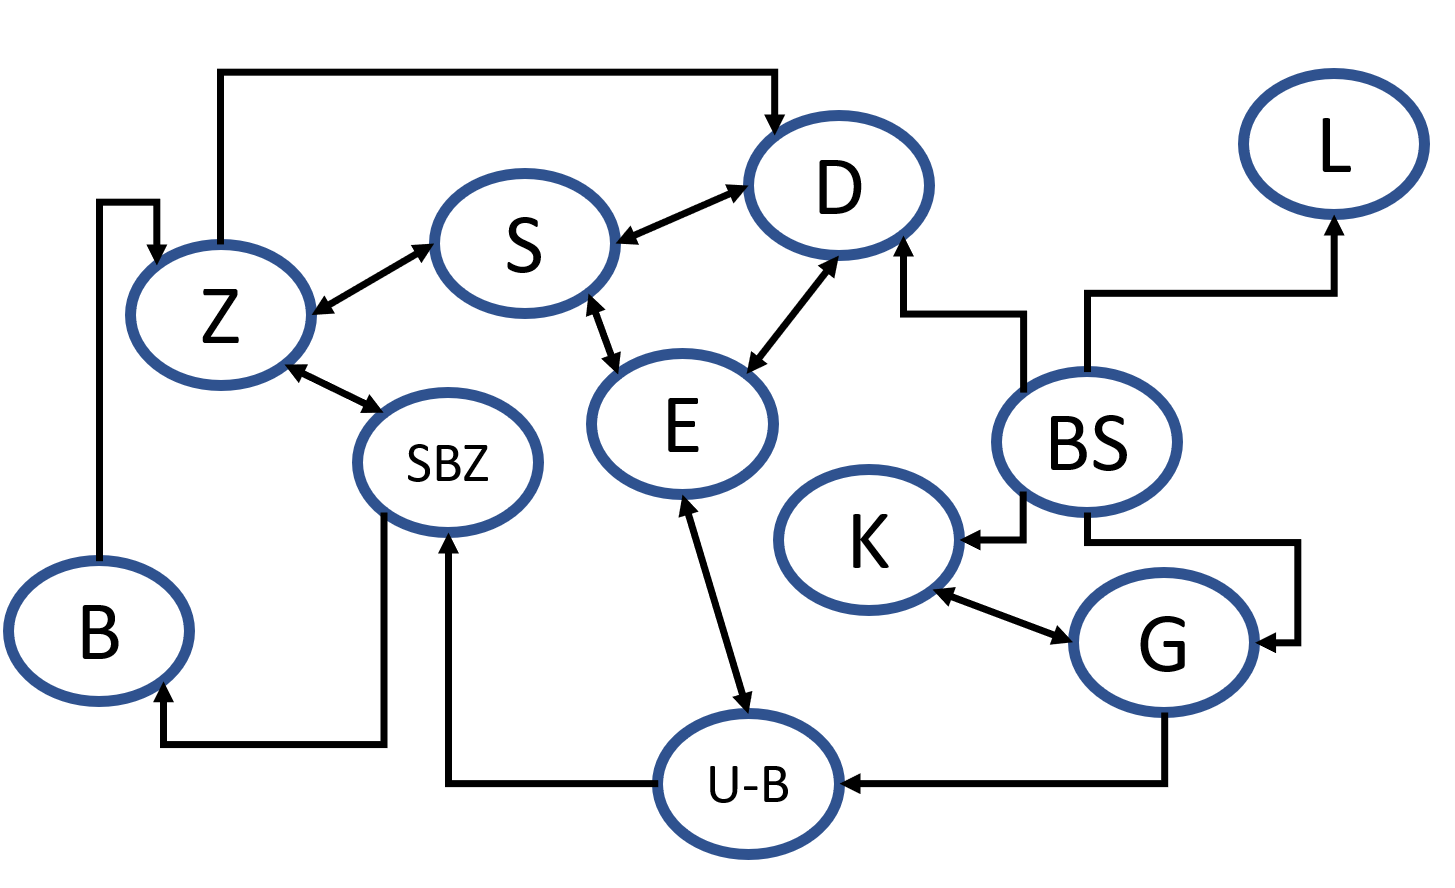
\includegraphics[width=\textwidth]{Pictures/Wikipedia.PNG} 
    \caption{Die Verlinkung von Wikipedia-Artikeln als Graphen.}
    \label{fig:wikipedia_graph}
\end{figure}

Wenn er anch dem Breitensuchealgorithmus vorgeht, wird er den Startartikel im Browser aufmachen (\textit{Breitensuche}, in unserem Beispiel von vorher) und dann jeden Link (\textit{Deutschland}, \textit{Graph}, \textit{Laufzeit}, \textit{Knoten}) in einem neuen Tab öffnen und anschliessend den Tab mit der Breitensuche schliessen. All die Artikel, die er jetzt im Browser offen hat, sind ein Klick vom Breitensucheartikel entfernt. Jetzt kann er dasselbe für den zuerst geöffneten noch offenen Tab (\textit{Deutschland}) tun. Er muss sich einfach merken, dass die neugeöffneten Tabs (\textit{Eisenbahn}, \textit{Schweiz}) sind jetzt 2 Klicks entfernt: Ein Klick mehr als die Seite, woher er kommt (\textit{Deutschland}). Er kann einfach für jedes Artikel aufschreiben, wie viele Klicks er vom Breitensucheartikel entfernt ist. Jeder nicht besuchter benachbarter Artikel wird ein Klick weiter sein.

\begin{aufgabe}\label{aufgabe_wikipedia_spiel}
Alice und Bob spielen das Wikipedia-Spiel auf den Graphen in Abbildung \ref{fig:wikipedia_graph}. Bob startet bei \textbf{BS} und muss in möglichst wenig Klicks \textbf{SBZ} erreichen. Helfe Bob herauszufinden, wie viele Klicks er braucht. Wie musst du den Breitensuchealgorithmus modifizieren, um die minimale Anzahl Klicks zu ermitteln? Führe deinen modifizierten Breitensuchealgorithmus auf diesen Graphen aus. Wie sehen in jedem Schritt \texttt{queue} und \texttt{visited} aus? Wo schreibst du die Abstände zwischen dem Startknoten und jedem besuchten Knoten auf?
\end{aufgabe}

\paragraph{Abstand zwischen zwei Knoten in Python ausrechnen}
Die Aufgabe \ref{aufgabe_wikipedia_spiel} hat mehrere möglichen Lösungen. Wir werden eine der Varianten in Python implementieren. In dieser Variante werden wir die Abstände genau dort speichern, wo wir sie brauchen: in der Warteschlange. Grundsätzlich gibt es zwei grosse Änderungen:
\begin{enumerate}
    \item Die Warteschlange enthält nicht nur Knoten, sondern auch deren Abstand vom Startknoten.
    \item Das Programm gibt anstatt von der Liste aller besuchten Knoten den Abstand zwischen Start- und Endknoten zurück.
\end{enumerate}

\begin{figure}[H]
    \centering
    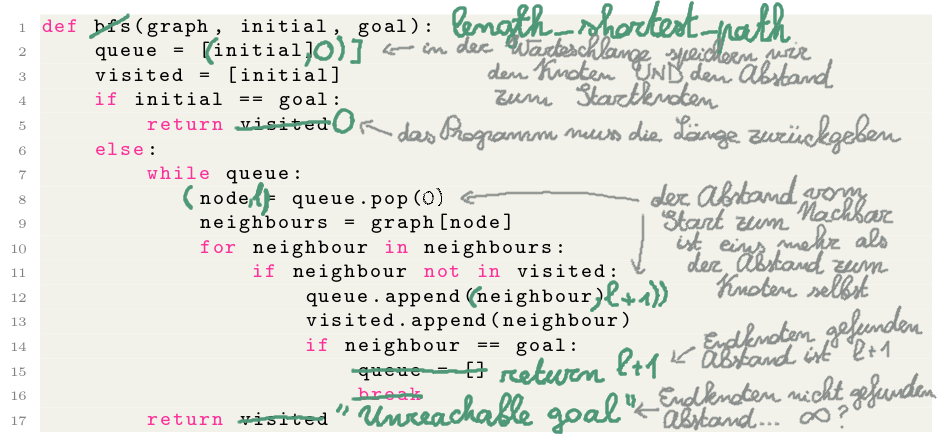
\includegraphics[width=\textwidth]{Pictures/SP/bfs_goal-to-length.png}
    \caption{Programm, das einen bestimmten Knoten sucht, in ein Programm umschreiben, das den Abstand zwischen Start- und Endknoten findet.}
    \label{fig:bfs_goal_to_length}
\end{figure}

\begin{lstlisting}[language=Python, caption={Programm, das den Abstand zwischen \texttt{initial} und \texttt{goal} berechnet.}, label={lst:length_shortest_path}]
def length_shortest_path(graph, initial, goal):
    queue = [(initial, 0)]
    visited = [initial]
    if initial == goal:
        return 0
    else:
        while queue:
            (node, length) = queue.pop(0)
            newlength = length + 1
            neighbours = graph[node]
            for neighbour in neighbours:
                if neighbour not in visited:
                    queue.append((neighbour, newlength))
                    visited.append(neighbour)
                    if neighbour == goal:
                        return newlength
        return "There is no path between initial and goal in the given graph"
\end{lstlisting}

\paragraph{Über wie vielen Ecken kennt jeder jeden?}
Alice hat gehört, dass jeder jeden über 6,6 Ecken kennt. Sie ist von dieser Theorie sehr begeistert und möchte herausfinden über wie vielen Ecken sie eine Person kennt, die schon Mal von einem Panda gebissen worden ist.

\begin{aufgabe}\label{aufgabe_panda_gebissen}
Hier ist eine Beschreibung von den Freundschaften von Alice und ihren Freunden.
\begin{displayquote}
Bob ist der beste Freund von Alice. Bob kennt ausserdem Charlie und David. Charlie, Elisabeth und Fred sind sehr eng befreundet und essen zusammen Kuchen jedes Wochenende. Fred und Alice kennen beide Gregory. Gregory und Hannah haben dieselbe Primarschule besucht und waren mit Jakob in einer Klasse. Jakob hat Fred im Militär kennengelernt. Jakob hat eine Schwester namens Lucy, und sie wurde einmal von einem Panda gebissen, als sie mit einer Bambushandtasche ins Zoo ging.
\end{displayquote}

\begin{enumerate}[(a)]
    \item Formalisiere die Freundschaften von Alice und ihrer Freunden als Graphen. Was sind die Knoten? Wann sind zwei Knoten durch eine Kante verbunden? Ist der Graph gerichtet oder ungerichtet?
    \item Führe den modifizierten Breitensuchealgorithmus aus, um den Abstand im Freundschaftsgraphen zwischen Alice und Lucy zu bestimmen.
    \item Stelle den Freundschaftsgraphen in Python als Liste der Nachbarn dar.
    \item Führe das Programm \ref{lst:length_shortest_path} auf dem Freundschaftsgraphen aus. Wähle Start- und Endknoten so, dass der Abstand (im Graphen) am grössten ist. Über wie vielen Ecken kennt jeder jeden in diesem Freundschaftsgraphen? 
\end{enumerate}

\end{aufgabe}

\paragraph{Norbert, der Staubsauger-Roboter}
Norbert ist ein alter Staubsauger-Roboter. Er putzt das Zimmer den ganzen Tag und nun hat er fast kein Akku mehr.
\begin{wrapfigure}{l}{0.5\textwidth}
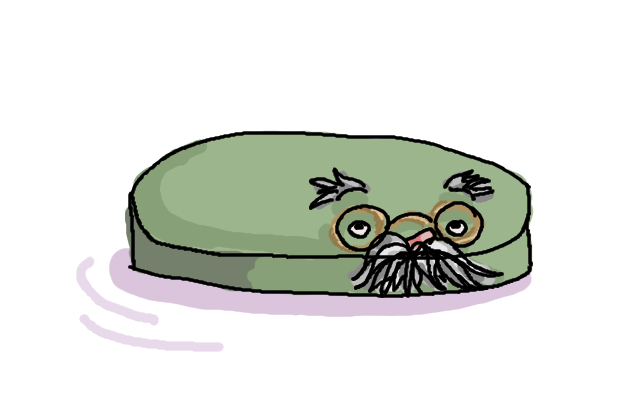
\includegraphics[width=0.9\linewidth]{Pictures/SP/norbert.png} 
\label{fig:norbert}
\end{wrapfigure}
Deswegen muss er so schnell wie möglich zurück zur Aufladestation.
Das Zimmer ist gefliest und Norbert kann von einer Fliese auf die andere fahren (das nennt er Schritt), aber nur nach vorne, hinden, links oder rechts, weil er sich nur um 90 Grad drehen kann. Ausserdem stehen im Zimmer Möbel herum, unter welchen Norbert nicht passt. Wie viele Schritte muss er bis zur Aufladestation fahren?

Norbert hat eine ziemlich gute mentale Karte vom Zimmer. Er weiss, dass das Zimmer 8 mal 6 Fliesen gross ist und einige grosse Schränke, Bücherregale und Sofas enthält. Er weiss genau, wo jedes Möbelstück steht.
\begin{figure}[H]
    \centering
    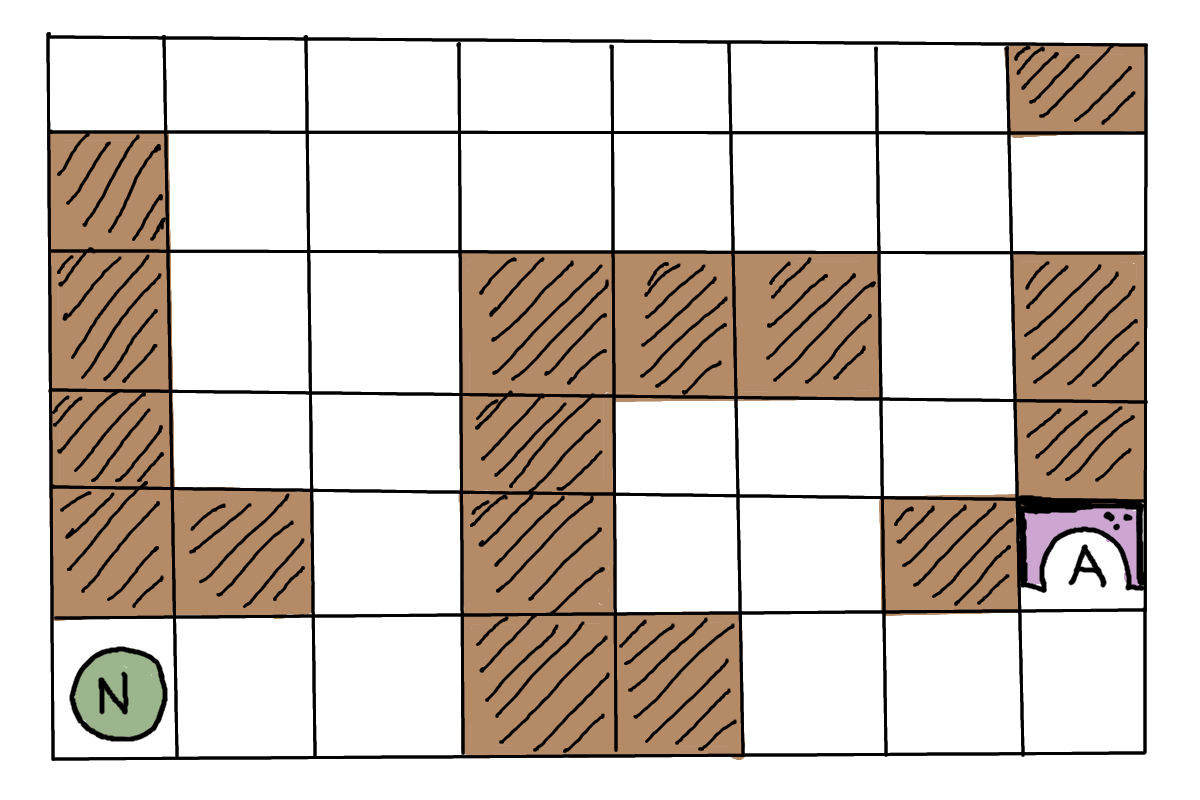
\includegraphics[width=\textwidth]{Pictures/SP/norbert_zimmer.png}
    \caption{Das Zimmer, wo sich Norbert befindet. In braun sind die Möbel markiert, unter welchen Norbert nicht passt. Norbert ist unten links, die Aufladestation ist unten rechts.}
    \label{fig:norbert_zimmer}
\end{figure}
Wir werden jetzt das Zimmer als Graphen modellieren, so dass die Anzahl Schritte, die Norbert bis zur Aufladestation fahren muss, dem Abstand zwischen den Knoten \texttt{N} und \texttt{A} entspricht.

Die Knoten vom Zimmergraphen sind die Fliesen und es gibt genau dann eine Kante zwischen zwei Knoten, wenn Norbert von der einen Fliese bis zur anderen in einem seiner Schritten fahren kann. Die Möbel sind als Knoten ohne Kanten modelliert.
\begin{figure}[H]
    \centering
    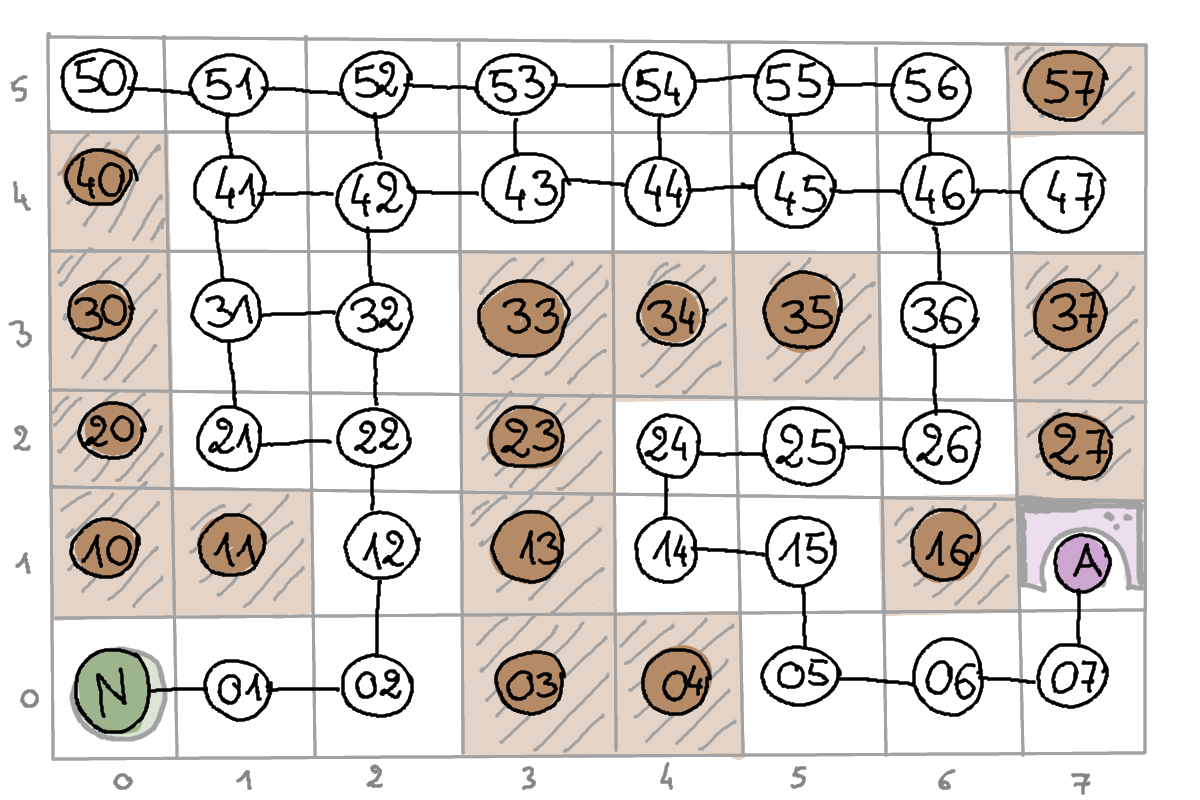
\includegraphics[width=\textwidth]{Pictures/SP/norbert_graph.png}
    \caption{Das Zimmer, wo sich Norbert befindet, als Graphen modelliert. Jede Fliese ist ein Knoten (mit deren Koordinaten als Name). Wenn Norbert in einem Schitt von einer Fliese zur anderen fahren kann, gibt es zwischen den entsprechenden Knoten eine Kante.}
    \label{fig:norbert_graph}
\end{figure}
Wir wissen schon, wie wir die Breitensuche benutzen können, um in einem solchen Graphen den Abstand zwischen \texttt{N} und \texttt{A} zu finden.
Die Knoten werden in Folgender Reihenfolge besucht und der gesuchte Abstand ist 17.
\begin{lstlisting}
visited = ["N", "01", "02", "12", "22", "21", "32", "31", "42", "41", "43", "52", "51","44", "53", "50", "45", "54", "46", "55", "36", "47", "56", "26", "25", "24", "14", "15", "05", "06", "07"]
\end{lstlisting}
Beobachte, dass die Möbelknoten gar nicht besucht worden sind, weil sie von \texttt{N} aus nicht erreichber sind.

\subsection{Der kürzeste Pfad}
Es ist sicher nützlich zu wissen, dass Bob in nur drei Klicks den Wikipedia-Artikel über den Zürcher Strassenbahnnetz erreichen kann, wenn der beim Breitensucheartikel startet; oder dass Alice über 3 Ecken jemanden kennt, der von einem Panda gebissen wurde; oder dass Norbert der Staubsauger-Rotober in 17 Schritten die Aufladestation erreichen kann. Aber wäre es nicht noch nützlicher zu wissen, welche Links muss Bob anklicken, oder welche Freunde und Freundesfreunde muss Alice kontaktieren, oder wo lang muss Norbert fahren?

Wir werden jetzt Norbert den Staubsauger-Roboter helfen, so schnell wie möglich seine Aufladestation zu erreichen. Wie auch für die Länge des kürzesten Pfades, gibt uns der Breitensuchealgorithmus alle benötigten Informationen, wir müssen sie nur speichern und richtig verwenden. Damit die Beschreibung ein Bisschen schneller geht, werden wir Norbert in ein kleineres Zimmer platzieren.
\begin{figure}[H]
    \centering
    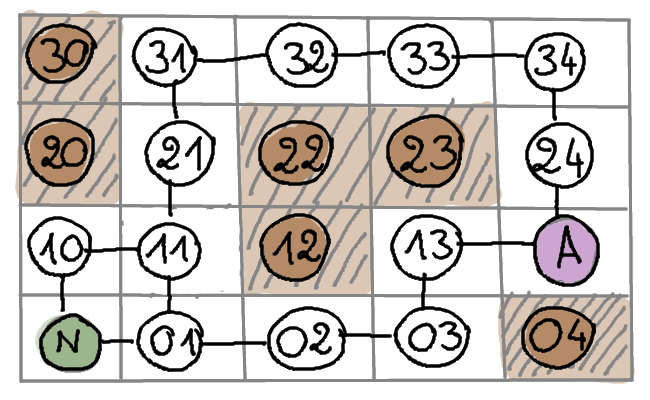
\includegraphics[width=0.6\textwidth]{Pictures/SP/norbert_klein_graph.png}
    \caption{Ein kleineres Zimmer für Norbert, schon als Graphen modelliert.}
    \label{fig:norbert_klein_graph}
\end{figure}
Nehmen wir an, wir führen jetzt die Breitensuche aus. Wir fangen bei \texttt{N} an und fügen \texttt{01} und \texttt{10} in die Warteschlange ein, weil sie die Nachbarn von \texttt{N} sind. Dann entfernen wir \texttt{01} aus der Warteschlange und fügen dessen Nachbarn hinzu: \texttt{02} und \texttt{11}. Wir machen so weiter, bis wir \texttt{A} gefunden haben.  Die Knoten werden in der folgenden Reihenfolge besucht.
\begin{lstlisting}[language=Python]
visited = ["N", "01", "10", "02", "11", "03", "21", "13", "31", "A"]
\end{lstlisting}
Aber wie können wir jetzt den Pfad ausrechnen?
Die wichtige Beobachtung ist, dass wir \texttt{A} als Nachbar von \texttt{13} gefunden haben. Das bedeutet, dass der kürzeste Pfad von \texttt{N} nach \texttt{A} über \texttt{13} verläuft. Wenn es einen kürzeren Pfad über einen anderen Knoten gegeben hätte, hätten wir \texttt{A} früher gefunden als Nachbar von einem anderen Knoten. Den Knoten \texttt{13} haben wir als Nachbar von \texttt{03} gefunden. Dann muss \texttt{03} auch auf dem kürzesten Pfad liegen. Den Knoten \texttt{03} haben wir von \texttt{02} gefunden, und \texttt{02} von \texttt{01}, und \texttt{01} von \texttt{N}.

Um den kürzesten Pfad aufzulisten haben wir die Nachbarn zurückverfolgt, von \textbf{A} zurück nach \texttt{N}, in der umgekehrten Reihenfolge, in der die Breitensuche sie gefunden hatte.
\begin{figure}[H]
    \centering
    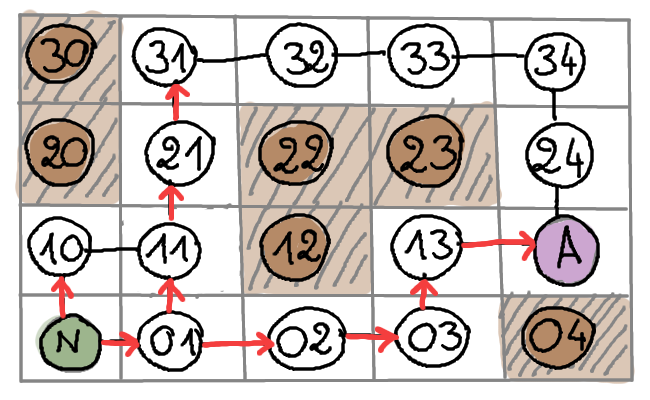
\includegraphics[width=0.6\textwidth]{Pictures/SP/norbert_klein_graph_arrows.png}
    \caption{Wir haben mit roten Pfeilen die Kanten markiert, die wir bei der Breitensuche verwendet hatten. Um den kürzesten Pfad von \texttt{N} nach \texttt{A} zu finden, müssen wir nur die Pfeile von \texttt{A} nach \texttt{N} zurückverfolgen.}
    \label{fig:norbert_klein_graph_arrows}
\end{figure}
Aus einem Knoten können mehrere rote Pfeile ausgehen (weil ein Knoten mehrere Nachbarn haben kann, die in die Warteschlange eingefügt werden), aber maximal ein Pfeil kann darauf zeigen (weil wir Knoten, die wir schon gesehen haben, kein zweites Mal in die Warteschlange einfügen). Alle rote Pfeile, wenn wir sie in die andere Richtung verfolgen, führen nach \texttt{N}, und zwar über den kürzesten Pfad.

\begin{aufgabe}\label{aufgabe_find_shortest_path}
Betrachte folgenden Graphen. 
\begin{figure}[H]
    \centering
    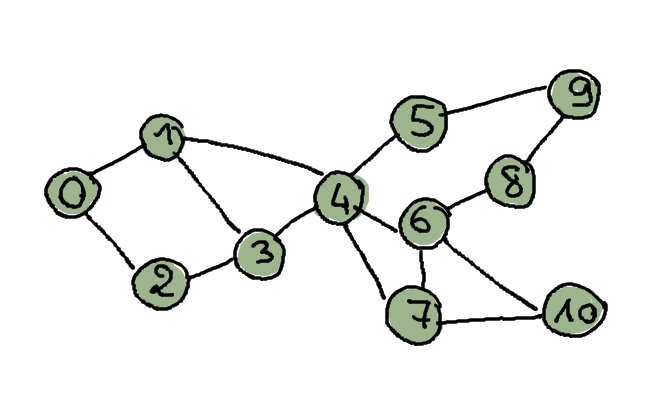
\includegraphics[width=0.6\textwidth]{Pictures/SP/shortest_path_graph.png}
\end{figure}
\begin{enumerate}[(a)]
    \item Finde den küzesten Pfad zwischen \texttt{0} und \texttt{9}. Benutze einen Breitensuche-ähnlichen Verfahren.
    \item Was würdest du machen, wenn du jetzt den kürzesten Pfad zwischen \texttt{0} und \texttt{10} finden müsstest? Kannst du etwas aus der vorherigen Teilaufgabe wiederverwenden?
    \item Wie würdest du den kürzesten Pfad zwischen \texttt{6} und \texttt{0} finden? Kannst du etwas aus den vorherigen Teilaufgaben wiederverwenden?
    \item Und wenn du den kürzesten Pfad zwischen \texttt{9} und \texttt{1} finden musst?
\end{enumerate}{}
\end{aufgabe}

\begin{aufgabe}\label{aufgabe_shortest_path_alg}
Überlege, wie du den Breitensuchealgorithmus verändern musst, um den kürzesten Pfad zwischen zwei Knoten zu finden. Du kannst deine Erkenntnisse aus Aufgabe \ref{aufgabe_find_shortest_path} benutzen.

Welche zusätzliche Informationen musst du speichen? Wo würdest du es machen?
Wie verwendest du diese zusätzliche Informatinen, um den Pfad zu finden?

Schreibe deinen Algorithmus möglichst genau auf.
\end{aufgabe}



\paragraph{Der kürzeste Pfad in Python}
Wir werden jetzt zusammen eine mögliche Lösung zur Aufgabe \ref{aufgabe_shortest_path_alg} in Python implementieren. Die zwei wichtigen Unterschiede zum ersten Breitensucheprogramm haben mit den roten Pfeilen aus Abbildung \ref{fig:norbert_klein_graph_arrows} zu tun:
\begin{enumerate}
    \item Wie wir die rote Pfeile speichern
    \item Wie wir die rote Pfeile zurückverfolgen
\end{enumerate}

Zuerst werden wir das erste Breitensucheprogramm so verändern, dass wir uns für jeden besuchten Knoten merken, woher wir diesen Knoten gefunden haben. Das Programm erwartet einen Graphen und einen Startknoten und gibt für jeden erreichbaren Knoten aus, woher wir diesen Knoten gefunden haben.

\begin{lstlisting}[language=Python, caption={Programm, welches die rote Pfeile ausgehend von einem Startknoten berechnet und ausgibt. Die einzigen zwei Zeilen, die sich verändert haben, sind 3 und 10.}, label={bfs_with_parent}]
def bfs_with_parent(graph, initial):
    queue = [initial]
    visited = {initial:None}
    while queue:
        node = queue.pop(0)
        neighbours = graph[node]
        for neighbour in neighbours:
            if neighbour not in visited:
                queue.append(neighbour)
                visited[neighbour] = node
    return visited
\end{lstlisting}

Führe das Programm auf den Graphen aus der Aufgabe \ref{aufgabe_find_shortest_path} aus. Kannst du alle rote Pfeile in der Ausgabe wieder finden?
\begin{lstlisting}[language=Python]
numbers = {0: [1, 2],
        1: [0, 3, 4],
        2: [0, 3],
        3: [1, 2, 4],
        4: [1, 3, 5, 6, 7],
        5: [4, 9],
        6: [4, 7, 8, 10],
        7: [4, 6, 10],
        8: [6, 9],
        9: [5, 8],
        10:[6, 7]}

print(bfs_with_parent(numbers, 0))
{0: None, 1: 0, 2: 0, 3: 1, 4: 1, 5: 4, 6: 4, 7: 4, 8: 6, 9: 5, 10: 6}
\end{lstlisting}

Jetzt schreiben wir ein Programm, das die roten Pfeile zurückverfolgt. Das Programm erwartet einen Startknoten, einen Endknoten und etwas in der gleichen Form, wie die Ausgabe von \texttt{bfs\_with\_parent}, und gibt den kürzesten Pfad zurück.
 
Stell dir vor, du hättest ein Buch von einer Person ausgeliehen, die du über 6 Ecken kennst. Du weisst nicht, wer diese Person ist und wo sie wohnt. Du weisst nur, wer dir dieses Buch gegeben hat. Und die Person, die es dir gegeben hat, weiss auch nur von wem sie es bekommen hat. Und so könnt du und deine Freunde die Kette bis zum Besitzer des Buches zurückverfolgen, der das Buch von niemanden bekommen hat und deswegen das Buch behält. Die Datenstruktur, die das Backtracking-Programm erwartet, speichert genau diese Relation: wer von wem das Buch bekommen hat.

\begin{lstlisting}[language=Python, caption={Programm, welches rote Pfeile zurückverfolgt}, label={backtracking}]
def backtracking(parents, goal):
    reversed_path = []
    node = goal
    while node != None:
        reversed_path.append(node)
        node = parents[node]
    return list(reversed(reversed_path))
\end{lstlisting}

\begin{aufgabe}\label{aufgabe_shortest_path}
Schreibe ein Programm in Python, welches, gegeben ein Graph, ein Start- und ein Endknoten, den kürzesten Pfad zwischen Start- und Endknoten ausgibt. Du kannst dafür \texttt{bfs\_with\_parent} und \texttt{backtracking} verwenden.
\end{aufgabe}

\paragraph{Ein Spaziergang im All}
\begin{figure}[H]
    \centering
    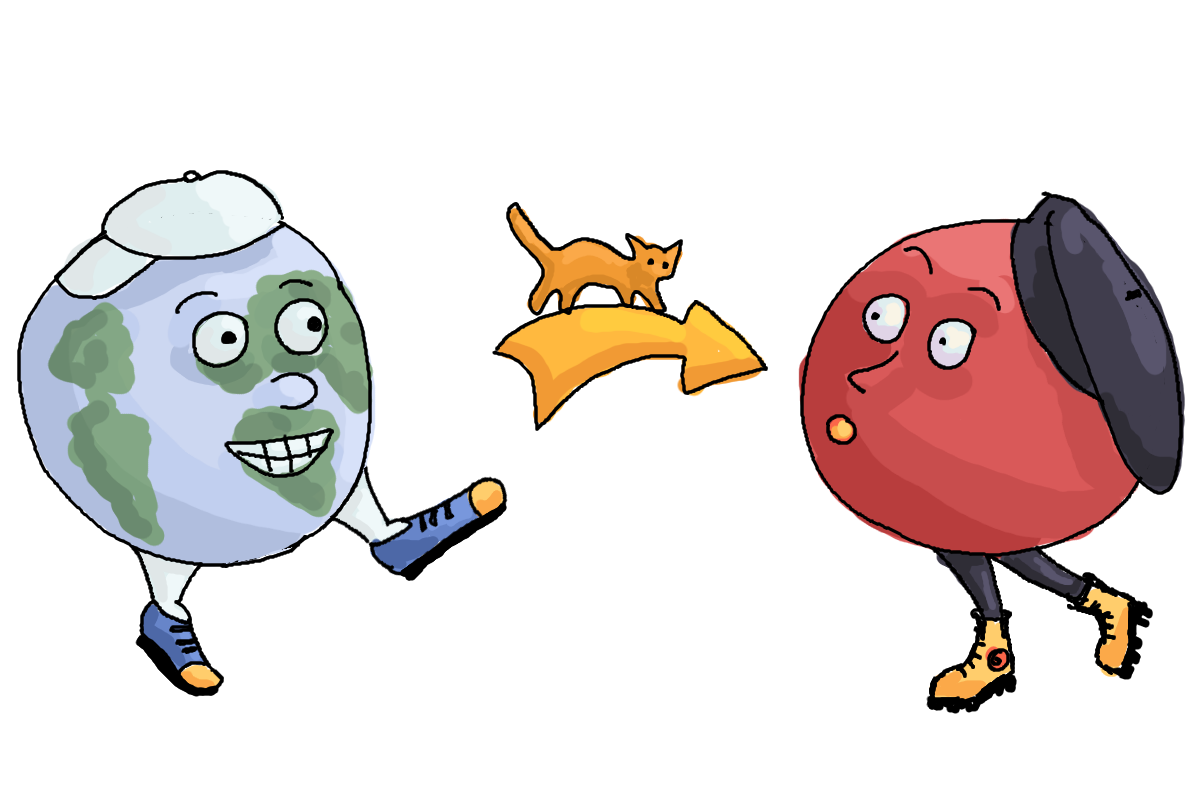
\includegraphics[width=\textwidth]{Pictures/SP/erde_mars.png}
\end{figure}
Wie weit ist es von der Erde bis zum Mars? Es kommt darauf an, wie man es misst! Wir behaupten, dass der Abstand kleiner oder gleich 12 sein muss. Und wie weit ist es von der Hand bis zum Fuss?
\begin{lstlisting}
HAND - FAND - FANS - FASS - FUSS
\end{lstlisting}
Der Sinn vom Spiel ist eine möglichst kurze Folge von Wörter zu finden, die das Start- mit dem Zielwort verbindet, wobei alle Wörter genau 4 Buchstaben haben und zwei Wörter dürfen genau dann daneben stehen, wenn sie sich genau um einen Buchstaben unterscheiden.


\begin{aufgabe}
\begin{enumerate}[(a)]\label{aufgabe_erde_mars_graph}
    \item Formuliere das Spiel als Graphen. Was sind die Knoten? Wann gibt es eine Kante zwischen zwei Knoten? Ist der Graph gerichtet oder ungerichtet?
    \item Zeichne den Graphen, der folgende Wörter modelliert:
    \begin{lstlisting}
    BANK, ZINS, ZANK, SINN, SAND, ZINK, SANK, ZINN
    \end{lstlisting}
    \item Füge zwei Wörter hinzu.
    \item Gibt es einen Pfad zwischen \texttt{BANK} und \texttt{ZINS}, welcher nur aus den aufgelisteten Wörter besteht?
    \item Wenn du das Wort \texttt{ZINK} entfenst, kannst du zwei Wörter hinzufügen, so dass \texttt{BANK} und \texttt{ZINS} immer noch verbunden sind?
\end{enumerate}

\end{aufgabe}

\begin{figure}[H]
    \centering
    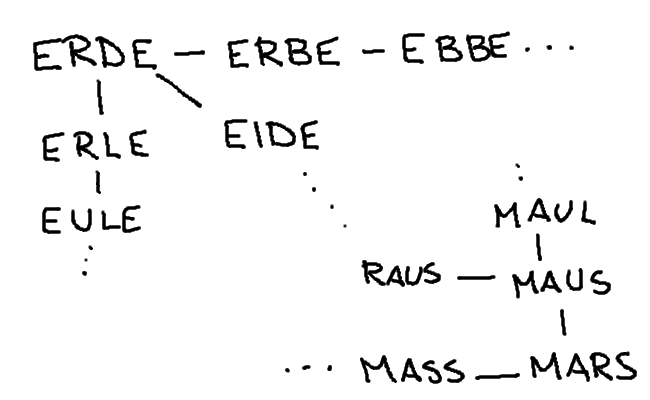
\includegraphics[width=\textwidth]{Pictures/SP/erde_mars_first_graph.png}
\end{figure}

\begin{aufgabe}\label{aufgabe_erde_mars_neighbours}
\begin{enumerate}[(a)]
    \item Schreibe den Graphen über den folgenden Wörter in der Liste der Nachbarn Darstellung.
    \begin{lstlisting}
    ERDE, EIDE, EINE, EINS, ZINS, ZINK, ZANK, ZACK, PACK, PARK, MARK, MARS,
    MAUS, HAUS, HASS, BASS, PARD, BAND, SAND, SACK, BANK, SANK, SINN, ZNINN,
    ZICK, PINS, EILT, EILE, EULE, ERLE, ENTE, ENDE
    \end{lstlisting}
    \item Rufe das Programm aus der Aufgabe \ref{aufgabe_shortest_path} auf und finde den kürzesten Pfad zwischen Erde und Mars heraus.
    \item * Du hast bestimmt bemerkt, wie mühsam und fehleranfällig es ist, solche Graphen selber zu konstruieren und zu erweitern. Dabei ist die Idee dahinter ziemlich einfach: Nachbarwörter unterscheiden sich um einen Buchstaben. Verwende deine Kenntnisse in der Stringmanipulation und Stringkomposition, um ein Programm zu schreiben, das eine Menge von Wörter und ein Wort erwartet und alle Nachbarwörter des Wortes ausgibt, die in der Menge der Referenzwörter enthalten sind.
    \item * Schreibe das Programm aus der Aufgabe \ref{aufgabe_shortest_path} so um, dass es den Graphen nicht als Liste der Nachbarn erwartet, sondern als Liste aller Knoten, und verwende dein Programm aus der vorherigen Teilaufgabe, um die Nachbarn zu berechnen.
    \item * Wäre es möglich auch für die Zimmer von Norbert dem Staubsauger-Roboter eine solche Darstellung zu verwenden? Schreibe das Programm, welches aus der Zimmergrösse und Möbelkoordinaten die Nachbarn von einem Knoten berechnet.
\end{enumerate}
\end{aufgabe}
Jetzt können wir noch mehr Wörter hinzufügen und herausfinden, was weiter von der Erde ist: der Mond oder der Mars.

\paragraph{Schlangenspiel}
Alice und Bob sind zufällig in den Kinderabteil eines Zuges gelandet. Auf dem Tisch ist ein Schlangenspiel gezeichnet.
\begin{figure}[H]
    \centering
    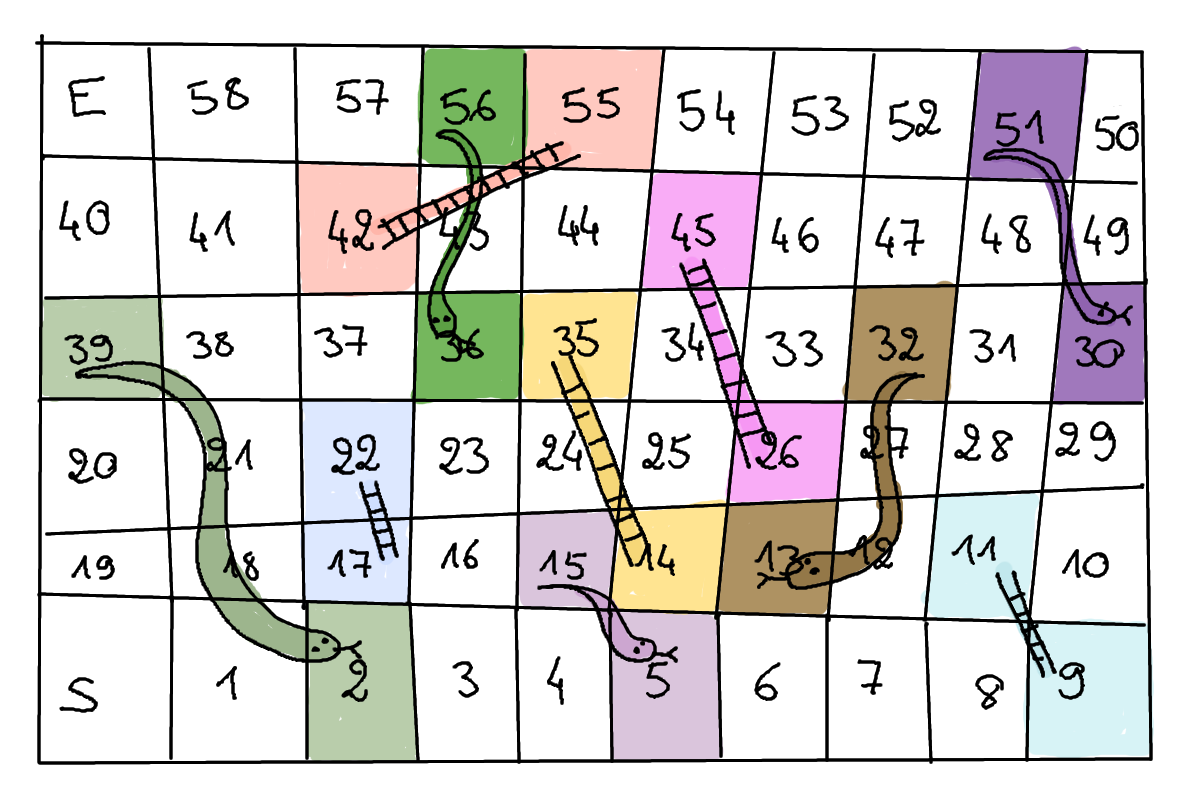
\includegraphics[width=\textwidth]{Pictures/SP/snakes_ladders_big.png}
\end{figure}
Sie haben zwar keinen Würfel, aber sie verwenden zwei Münzen, um einen Würfel mit 4 Seiten zu simulieren (zum Beispiel, \texttt{(KOPF, ZAHL)} entspricht einer 1, \texttt{(ZAHL, KOPF)} einer 2, \texttt{(ZAHL, ZAHL)} einer 3 und \texttt{(KOPF, KOPF)} einer 4).
Bob will um jeden Preis gewinnen. Er hat schon herausgefunden, wie er die Resultate seiner Münzenwürfe steuert. Aber er weiss nicht, welche Zahlen rauskommen müssen, damit er mit möglichst wenig Münzenwürfe das Ziel erreicht.

\begin{aufgabe}\label{aufgabe_schlangenspiel}
Zunächst werden wir mit einem kleineren Spielfeld arbeiten.
\begin{figure}[H]
    \centering
    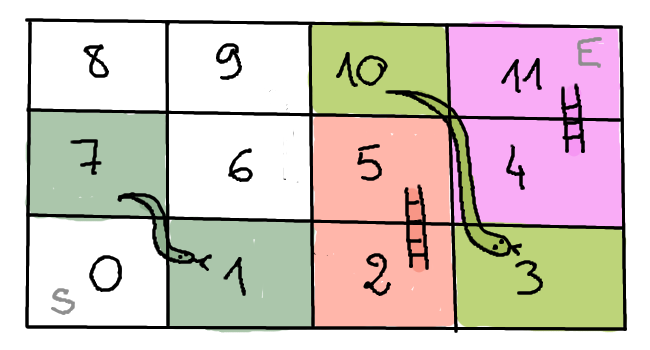
\includegraphics[width=\textwidth]{Pictures/SP/schlangen_spiel.png}
\end{figure}
\begin{enumerate}[(a)]
    \item Formalisiere das Schlangenspiel als Graphen. Was sind die Knoten? Wann gibt es eine Kante zwischen zwei Knoten? Ist der Graph gerichtet oder ungerichtet?
    \item Schreibe das kleinere Spielfeld in der Liste der Nachbarn Darstellung.
    \item Was muss Bob würfeln, um zu gewinnen? Führe das Programm aus der Aufgabe \ref{aufgabe_shortest_path} aus.
    \item Schreibe das Programm aus der Aufgabe \ref{aufgabe_shortest_path} so um, dass es die Zahlen ausgibt (1, 2, 3, 4), die Bob erzielen muss.
    \item * Überlege, was du brauchst, um die Nachbarn zu berechnen. Schreib ein Programm, welches alle Nachbarn von einem Knoten ausgibt.
    \item * Kombiniere deine Programme aus den vorherigen Teilaufgaben und helfe Bob das Schlangenspiel auf dem grossen Spielfeld zu gewinnen. Was muss er würfeln?
\end{enumerate}{}
\end{aufgabe}
